\documentclass[conference]{IEEEtran}
\IEEEoverridecommandlockouts
% The preceding line is only needed to identify funding in the first footnote. If that is unneeded, please comment it out.
\usepackage{cite}
\usepackage{amsmath,amssymb,amsfonts}
\usepackage{algorithmic}
\usepackage{graphicx}
\usepackage{textcomp}
\usepackage{array}
\usepackage{tabularx}
\usepackage{multirow}
\usepackage{xcolor}
\def\BibTeX{{\rm B\kern-.05em{\sc i\kern-.025em b}\kern-.08em
    T\kern-.1667em\lower.7ex\hbox{E}\kern-.125emX}}
\begin{document}

\title{ARShield: Protecting Users Against Clickjacking Attacks in Augmented Reality}

\author{\IEEEauthorblockN{Ani Avetian}
\IEEEauthorblockA{\textit{M.S. Computer Science and Software Engineering} \\
\textit{University of Washington}\\
Bothell, Washington \\
avetian7@uw.edu}
}


\maketitle

\begin{abstract}
Virtual reality (VR) and augmented reality (AR) devices are slowly taking over the market. With companies advocating for a future that relies heavily on a more virtual world, one questions how safe these environments can be. Previous work has looked at the security and privacy of AR devices and proposed different methods to keep people safe from malicious attackers. However, no work has looked into solutions specifically around clickjacking attacks in the AR environment. Clickjacking is when a user clicks something, generally on a webpage, and the action taken by that click is not what the user intended but potentially a malicious action put in by a malicious user. Most research has looked at clickjacking on web browsers as it is more common in these spaces. In this paper, we will specifically look at clickjacking attacks in ARKit and RealityKit, Apple's software development kits for creating AR applications. We will develop a solution for clickjacking attacks using computer vision algorithms and test it on an AR iOS application called ARShield. Using CreateML, we developed two different machine learning (ML) algorithms, an object detection and an image detection algorithm to detect clickjacking. We integrated the image detection algorithm into ARShield as it had a higher level of accuracy during the training, validation, and testing stages. While object detection had a lower accuracy rate overall. With this experiment we are able to provide strong evidence that image detection algorithms can in fact detect clickjacking within the AR space. This can be used as a first step to developing a better more intricate solution towards clickjacking in more AR spaces, not limited to Apple's development environment. 

\end{abstract}

\begin{IEEEkeywords}
clickjacking, augmented reality, computer vision, image recognition
\end{IEEEkeywords}

\section{Introduction/Background}

Virtual Reality(VR) and Augmented Reality(AR) devices seem to be gaining popularity as the years go by. These technologies, which once were just an idea, are now being integrated into our day-to-day lives. So what are these VR and AR technologies? VR is a simulated experience where a person is fully immersed in a virtual world whereas AR is a simulated experience where a person sees content overlaid on the real world. 

One of the most notable AR devices was the Google Glass. The device allowed you to live-stream video, take photos, get live directions to your destination, and  get text translations in real-time \cite{colin_steele_what_nodate}. The device was ahead of its time when it launched in 2013 and because of that, a lot of security concerns came up. For example, one was how the glasses were always recording a persons activities \cite{colin_steele_what_nodate}. Due to many concerns surrounding privacy and the fact that technology has changed so much, the Google Glasses are not being sold anymore. 

Mobile applications have also made use of AR technology, most notably the game Pokémon Go, launched in July 2016 \cite{paavilainen_pokemon_2017}. The location-based AR application used a player's camera to find Pokémon in the real world and once found the Pokémon characters would be shown as an overlay on the player screen to be interacted with \cite{paavilainen_pokemon_2017}. 

Headsets that combine AR/VR have also been gaining popularity. Meta's Quest Pro is at the forefront of using VR. The headset allows one to be fully immersed in a world called the metaverse. In the metaverse, a person can shop, interact with others, and play games, practically living their life out in the virtual world \cite{wang_survey_2023}. A person can also switch to using an AR mode that seemingly incorporates virtual objects in the real world. Microsoft's HoloLens is another great example of the innovations of AR and most recently Apple's Vision Pro headset is the newest addition to the family of headsets. 

With all this new technology, one must question the risks they pose. Specifically within cybersecurity. What kinds of attacks can be carried out by malicious actors in these virtual and augmented worlds? What security and privacy concerns should be addressed? Are there systems in place to make sure users are protected while using VR and AR? 

In this paper one specific concern we will look at is clickjacking within the AR space. To define clickjacking we must look at it in an a web browsing environment as this is where clickjacking is likely to occur. Clickjacking is a way an attacker can lure a victim to click an element on a page that will do what the attacker wants it to do, not what the user believes the element can do\cite{balduzzi_solution_2010}. This is generally done with an invisible layer placed behind the front facing website that will conduct the malicious act. For example, a user could be browsing a website and see a button saying "Click here for free dinner recipes". However, an attacker could have placed an invisible layer under the button that will instead trigger something on a malicous website instead of giving you free recipes. 

Clickjacking is not only found on web pages, it can happen within an AR environment where 3D objects are placed on top of one another. When a user interacts with an object they could potentially be interacting with something malicious underneath. Since AR systems are so new, there are not many solutions or detection algorithms built to identify clickjacking. The AR system that we will look at specifically is ARKit and RealityKit. These are Apple's software development kits that allows for developers to create their own AR supported iOS applications \cite{inc_augmented_nodate}. Within these development kits lies a vulnerability where if two objects are the same size, shape, and are overlaid on top of each other, a clickjacking attack can occur. This is the vulnerability we will try to protect against in this paper.

In this paper we will develop computer vision algorithms that will detect whether an object has another layer underneath, potentially signifying a clickjacking attack. This will protect users and keep them secure while they are using any AR device. Its important to look at these scenarios as AR devices are gaining popularity and soon could become more integrated with our lives. 

This paper will also discuss work related to this area followed by the design of our current solution. We will discuss results and conclude with further research in this area. 

\section{Related Work}

\subsection{Threats to VR/AR Environments}

With the increase of VR/AR devices and the push from companies to use them, there are still threats that need to be fully explored and vulnerabilities to be mitigated. Even though this paper specifically looks at clickjacking other threats do exist. 

Several papers have looked into some of these issues and how easy it can be to attack a user in an VR/AR environment. One paper looked into keylogging based on a users head motions \cite{slocum_going_nodate}. Others have looked at how monitoring hand gestures can be used to guess credentials typed in \cite{gopal_hidden_nodate}. For both of these studies, there was high success rates in the models built to do these attacks. 

Other papers have looked at more novel threats to security and privacy. For example, any output rendered by the AR device needs to be secured \cite{dissanayake_review_2018}. Its important to understand that AR devices constantly monitor the world around you and collect data on your surroundings to generate 3D objects \cite{dissanayake_review_2018}. This data must be protected. 

\subsection{Clickjacking}

Clickjacking is not a new concept. Research has looked into what clickjacking is and its defences. The most common place we see clickjacking is within web browsers\cite{huang_clickjacking_nodate}. Generally an attacker would present a user interface (UI) element to a user in hopes the user will interact with it. However, once iteracted with the UI element may contain a hidden malicious action placed by the attacker. For web browsers many solutions exists like having users confirm on a popup what they want their action to do, the interface can randomize the UI layout, and in the most known method, we can disallow elements on a page to be rendered in iframes \cite{huang_clickjacking_nodate}. This basically disallows another HTML page to be rendered in the one you are currenly on. When it comes to AR, a lot of these novel solutions will not be applicable as we are not dealing with the same languages and frameworks. For example, there are no iframes in AR frameworks so disallowing them will do nothing. 

Previous studies have looked at clickjacking for AR browsers. AR browsers hold similar characteristics to normal AR apps since they overlay interactive elements on a users view of the world \cite{mcpherson_no_2015}. Its important to mention that these kinds of applications "amplify existing threats" that can be seen in normal web browsers, for example, clickjacking threats \cite{mcpherson_no_2015}. The paper suggested a solution that would look at the overlays of different objects on top of one another\cite{mcpherson_no_2015}. Specifically, creating and equivalent solution to web browser solutions like X-Frame-Option \cite{mcpherson_no_2015}. However, there was no actual solution built here. 

Another study looked specifically at clickjacking within ARKit. This study achieved a clickjacking attack by allowing two 3D objects to be placed at the same coordinates \cite{cheng_when_nodate}. Since ARKit has an inconsistency about which object is displayed first when they are on top of each other, it creates a vulnerability that an attacker can exploit \cite{cheng_when_nodate}. This paper successfully proved how easy it was to perform an attack like this and conclusions were drawn on possible mitigation's. For example, allowing users to interact with objects in AR when the object has been visible for a specific amount of time\cite{cheng_when_nodate}. However, because of the uncertainties within the 3D space, it is still unknown what will and will not work to defend against attacks like this \cite{cheng_when_nodate}.

Although not the same, cursorjacking is another avenue studied in AR. Cursorjacking is an attack that gradually moves the users cursor from what they want to click on to another malicious object\cite{su_perception_2022}. Experiments done in this area proved successful and its important to understand and defend against these kinds of attacks.

VR testing has also been studied. Even though AR and VR are different, a lot of the same strategies apply to both kinds of environments since they both work with 3D objects. One paper suggested a VR testing framework called VRTest\cite{wang_vrtest_2022}. This framework can be used to locate object in the virtual space\cite{wang_vrtest_2022}. 

\subsection{Computer Vision}

Computer vision algorithms are a type of artificial intelligence that allows users to get information from visual inputs such as photos and videos \cite{noauthor_what_nodate}. This type of algorithm is a subset of machine learning. In this paper we will be using this approach to build out an algorithm. This is not the first time computer vision has been used in the AR space. For example, the Apple Vision framework uses computer vision in their Core ML model to allow for object recognition. ARKit makes use of this framework as well. Users can even develop their own algorithms and use them within their apps for ARKit. Meta's AR devices also use computer vision algorithms to help estimate where the controllers positions are within the AR space, removing the need to use external tracking measures \cite{noauthor_how_nodate}. With technology getting better and better these algorithms have become more efficient as time goes on \cite{noauthor_how_nodate}.

\section{Design/Methodology}

\begin{figure*}[!t]
  \centering
  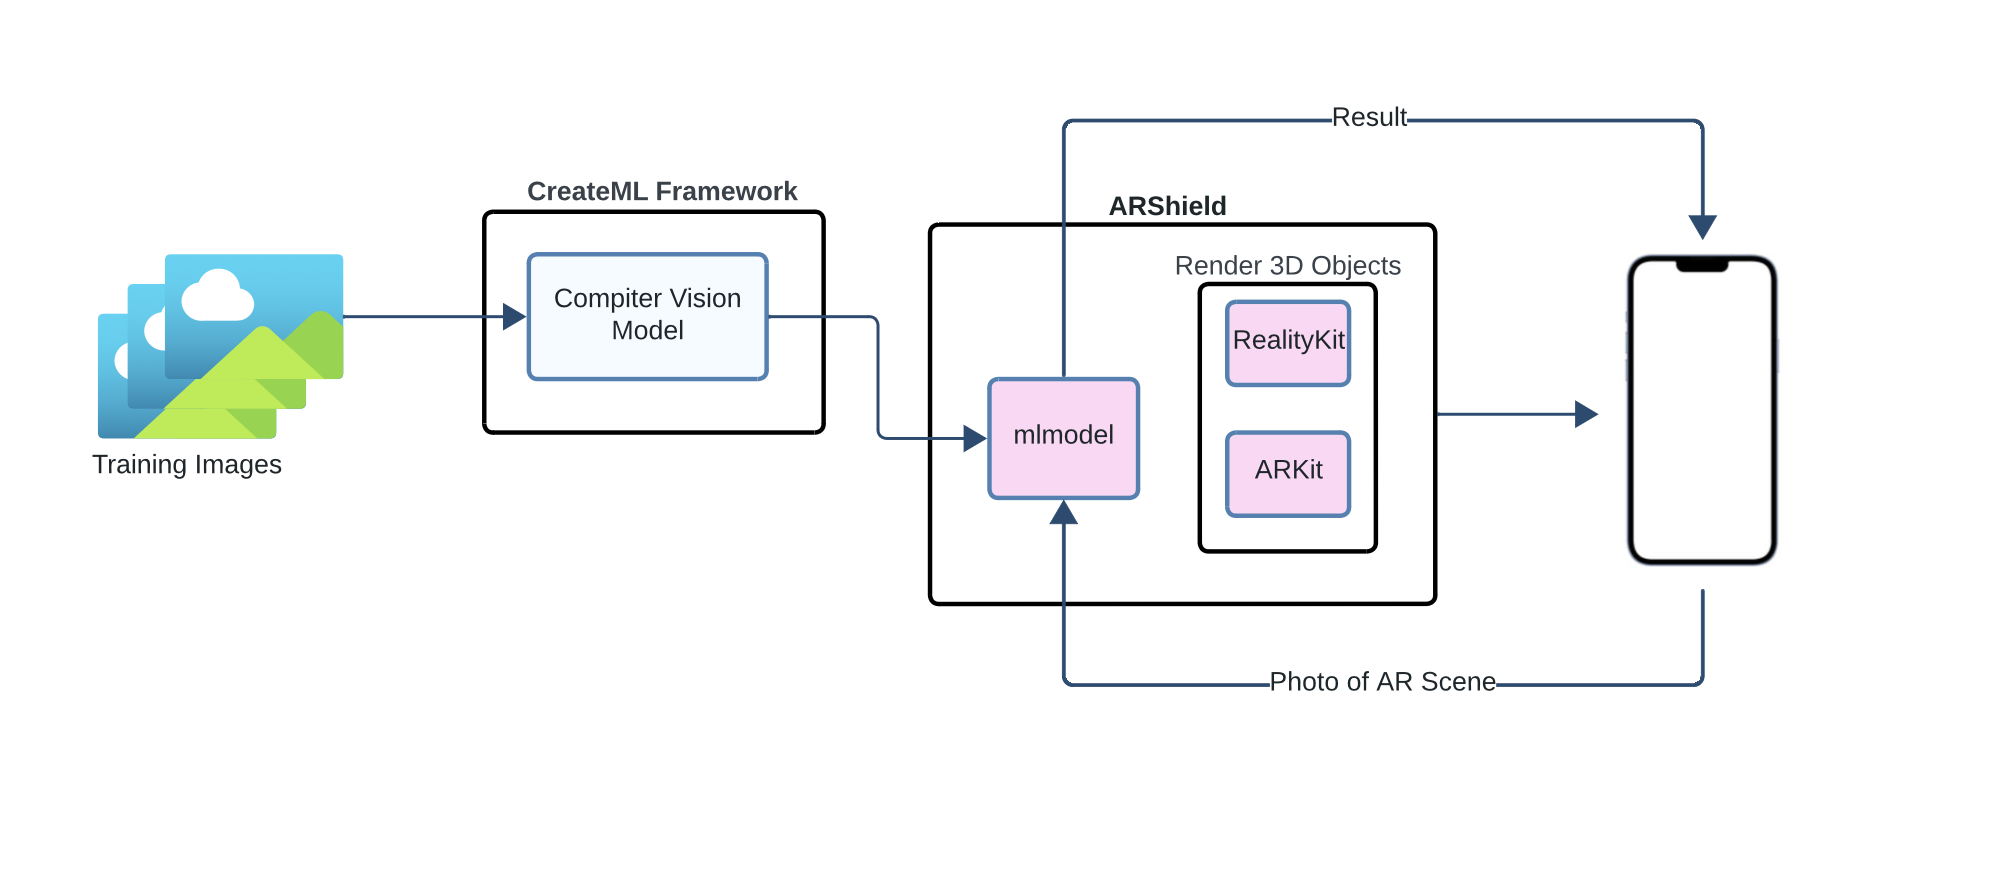
\includegraphics[width=\textwidth]{fig2.png}
  \caption{Architecture of Solution}
  \label{fig:example}
\end{figure*}

\subsection{Motivation}

The AR space is becoming more integrated with our lives with the release of more applications and devices that support it. With Apple's Vision Pro headset being one of the most recent launches of a VR/AR device, other companies will follow Apple's lead to create more in the VR/AR space. To ensure that users are not tricked into doing things they don't want to do, this research is important to conduct. Without user interactions, the AR space can be deemed useless and nothing would work as intended. Therefore, by defending against the very thing that makes AR usable we will allow for a safer and better AR experience. 

Additionally, there are no current solutions to these kinds of threats. With this paper, we aim to provide a possible solution to clickjacking attacks. 

\subsection{Clickjacking Design}

ARKit has a vulnerability where if two objects are the same size, shape, and are anchored on the same plane in the AR environment, one object can be completely concealed behind the other. This creates a vulnerability an attacker can exploit and use for a clickjacking attacks. This is the attack that we will simulate and try to defend against in this paper.  

\subsection{Threat Model}

To understand the threat model, we must understand the scenarios in which a clickjacking attack can occur: 

\begin{enumerate}
    \item An attacker making use of the AR object to advertise. Advertising in AR is a huge industry that is expected to grow tremendously in the coming years \cite{noauthor_ar_nodate}. An attacker can leverage vulnerabilities within ARKit, placing the advertisement below and object and a user can click on it.
    \item An attacker making use of AR objects in applications where something is intended to be hidden. For example, gaming applications may need things to be hidden \cite{cheng_when_nodate}. The attacker could be someone on the inside, placing a malicious item behind something. It could never be caught and an update would be rolled out to all players. 
    \item An attacker could leverage social engineering tactics to have a user click on an object they think is useful, but underneath it may not be what the user intended. For example, it can show something inappropriate to the user. 
\end{enumerate}

For all of these scenarios, we can assume the attacker has knowledge of the ARKit/RealityKit environment and the vulnerabilities that come with it. This way they know exactly how to exploit the system. The attacker will be someone who does have a malicious purpose of deceiving the user, making them do things they don't want to like click advertisements not necessary to them or potentially steal credentials if they are led to a malicious site when clicking an object. In all cases, it will be an attacker leveraging the vulnerability of placing objects behind one another, with the malicious action behind a real object. 

\subsection{System Model}

These types of attacks can be run on Apple devices that have the capability to run AR applications. The most common would be Apple iPhones. Since ARKit/RealityKit are development kits specifically built with Swift and SwiftUI, Apple's coding languages, these apps will be running only on Apple devices. An iPhone must be on iOS 11.0 or later and must be using an A9 or later processor \cite{noauthor_verifying_nodate}.

\subsection{User Model}

The users for this study range quite a bit. It can be people trying to just use the AR applications for their enjoyment or it can be developers creating AR applications. For people trying to just use the AR app, they could have concerns about how safe the environment is to interact with. They would not want unintended consequences of their interactions with objects. With developers, they would not want external users or advertisers placing objects on top or behind their own. As a developer, they would want the object placed in AR to do exactly what the object is intended to do. 


\subsection{Architecture}

In Figure 1 we can see an architecture of the experiment. Training photos of clickjacking attacks vs non-clickjacking attacks were collected. These images were annotated properly and classified for the machine learning model to read. Using the CreateML framework, Apple's framework to train ML models, the training photos along with testing photos were loaded in. Once a fully trained and tested model was ready, it was loaded into the ARShield application as a .mlmodel file. The code in ARShield could now be configured to use the ML model to make predictions. ARShield generates 3D objects using ARKit and RealityKit that can be moved around but initially spawn on top of each other. A photo of the AR scene can be fed into the ML model to do predictions of whether there is a clickjacking attack or not. The result is displayed to the user. Figure 2 shows an image of the UI of this application upon the initial load in. 

\begin{figure}
  \centering
  \includegraphics[width=150pt]{IMG_4308.PNG}
  \caption{Inital Load In For ARShield}
  \label{fig:example}
\end{figure}

\section{Implementation}

\subsection{ARShield: The ARKit/RealityKit Application}

Upon launch of the application you are shown multiple different elements. The main screen shows your AR environment. When the application initially loads, as seen in Figure 2, two objects resembling cubes are overlaid at the same exact position in the environment. Underneath the AR view is a button to take a photo of the environment a detection window is located to the left of the button. As a user, you can move the cubes from their initial placement to simulate what a clickjacking attack can look like. Figure 3 shows what clickjacking can look like where two objects are slightly overlaid on top of each other. Figure 4 shows what a normal set of objects may look like as the two cubes are not overlapping. In each photo we can see the detection shown at the bottom of the screen as to whether clickjacking was detected or not. This is because when the cubes are placed to the users liking and the "Take Photo" button is clicked, the image goes to the ML model to get classified as clickjacking or not. Depending on the classification, that alters the results shown to the user.

\begin{figure}
  \centering
  \includegraphics[width=150pt]{IMG_4310.PNG}
  \caption{Clickjacking Example}
  \label{fig:example}
\end{figure}

\begin{figure}
  \centering
  \includegraphics[width=150pt]{IMG_4311.PNG}
  \caption{Normal Example}
  \label{fig:example}
\end{figure}

\subsection{The Clickjacking Detection Model}

The clickjacking detection model used was an image detection model provided by CreateML. This image detection model was a feature extractor model. The model took in 50 training photos and 6 test cases. Once the model was trained in CreateML it was integrated into the application.

\subsection{Training Data}

There were a few testing scenarios used to train the model. These scenarios were built in Swift with the ARKit and RealityKit library. Screenshots were taken of the different testing scenarios to use as training data. The testing scenarios are as follows: 

\begin{enumerate}
    \item Testing on transparent objects where the malicious object can be seen behind the normal object.
    \item Testing on objects not directly on top of each other, where you can see the edges of the malicious one.
    \item Testing on malicious objects fully concealed behind another object.
    \item Testing on objects far away from each other, not being concealed, to show a normal case that's not clickjacking 
\end{enumerate}

These scenarios will be referenced as Test Case 1, 2, 3, and 4 in the rest of the paper. 

\subsection{Challenges}

Initially, we intended for an object detection algorithm to be used in this application instead of an image detection ML algorithm. The object detection model would use the You Only Look Once (YOLO) framework which is specific to object detection. However, there were many challenges with this model. Not only was it more difficult to train the model as each photo had to be annotated to be fed into the training set, but the model couldn't be integrated into the application. Even with numerous attempts, the application kept crashing when integrated due to buffer overflows in the app. It could not handle the detection being done on each frame of my AR environment. Therefore the code had to be reworked to fit an image detection model instead. Since this was the case, the user experience was affected. With object detection, the goal was to have the detection always happening in the background. With image detection, this is not possible. Image detection algorithms need to look at one photo at a time instead of objects being detected continuously. With the image detection algorithm integrated the user now has to take charge and take a photo each time they want to do clickjacking detection. 

\section{Results}

\subsection{Experimental Setup}

To set up the experiment locally use the guide located here: https://github.com/aniavetian/ARShield/. All instructions on the setup can be found to reproduce the clickjacking detection seen in ARShield. 

\subsection{The Results}

The purpose of this experiment was to look at computer vision models and their accuracy towards clickjacking. There was two models used throughout the entirety of this project, however only one was integrated into our application. Since both were trained we will present both results. 

A object detection model was initially trained for ARShield, but the integration of the model did not work causing us to switch gears to use an image detection model. The object detection model was also trained on CreateML, same as the image recognition model which was later integrated. Both models were trained on a series of 50 photos. 32 were clickjacking and 18 normal scenarios. The validation data was split from the training data and was not visible to us as it was auto split in CreateML.

\begin{table}[htbp]
    \centering
    \begin{tabular}{|c|c|c|c|}
        \hline
        Model & Training Accuracy & Validation Accuracy & Test Accuracy\\
        \hline
        Object Detection & 36\% & 29\% & 15\% \\
        Image Detection & 100\% & 80\% & 67\% \\
        \hline
    \end{tabular}
    \caption{Accuracy for ML Models}
    \label{tab:simple-table}
\end{table}

\begin{table}[htbp]
    \centering
    \begin{tabular}{|c|c|c|c|c|}
        \hline
        \# of Detection's & Test Case 1 & Test Case 2 & Test Case 3 & Test Case 4 \\
        \hline
        30 & 80\% & 83\% & 70\% & 100\% \\
        \hline
    \end{tabular}
    \caption{In-App Accuracy Testing for Image Detection Model}
    \label{tab:simple-table}
\end{table}

\begin{figure*}[!t]
  \centering
  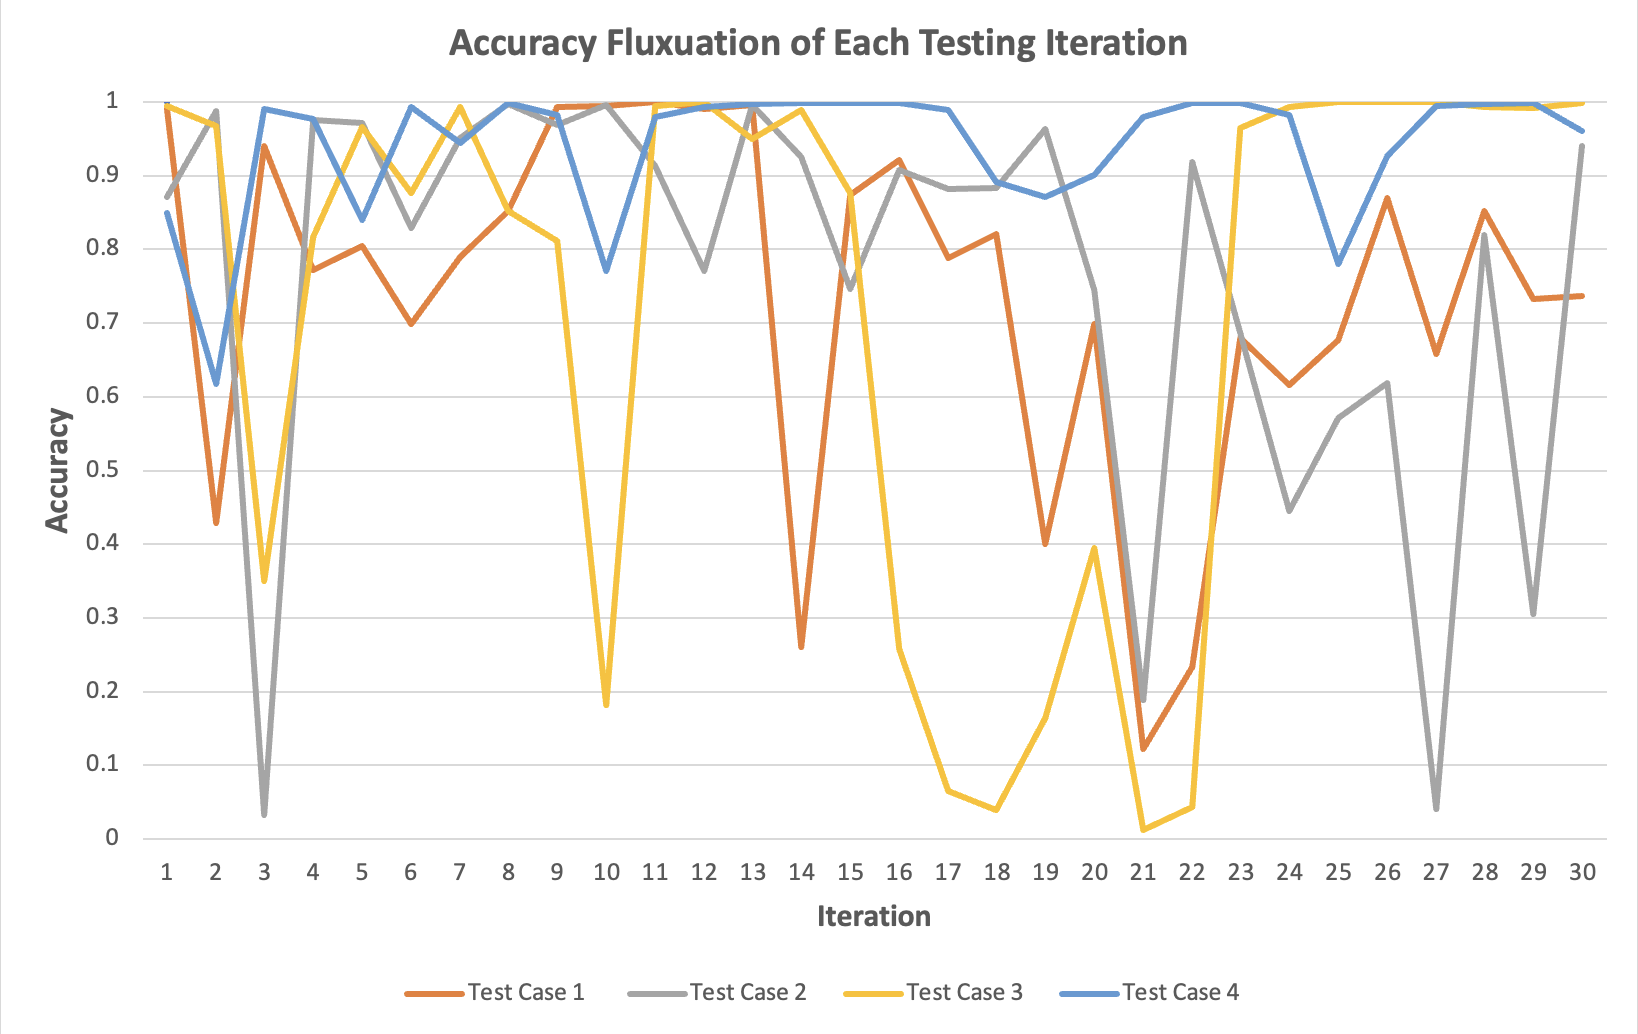
\includegraphics[width=\textwidth]{plot.png}
  \caption{Architecture of Solution}
  \label{fig:example}
\end{figure*}

In Table 1 we can see the results of the accuracy's given by the CreateML framework on its evaluation of the models. 

There was also in-app testing done where objects were moved in accordance to the training cases mentioned above. For each training case, the apps image detection was done numerous times to collect an average on whether the test case was correctly detected or not. The number of times was chosen arbitrarily. Additionally, to provide variance in the testing, the objects in the AR space were slightly moved for each time a detection was made. For test case 1 through 3 if the detection was shown as "Clickjacking" then that was deemed correct. For Test Case 4 if the detection was shown as "Normal" then that was deemed correct. The results are shown in Table 2. 

Figure 5 presents the accuracy as a line chart on each time the "Take Photo" button was clicked for the 30 times we collected data. Each line represents the different test cases done. The accuracy is measured in percent with 1 being 100\% accuracy and 0 being 0\% accuracy. The accuracy describes if the model guessed "Clickjacking" for Test Cases 1 through 3 and "Normal" for Test Case 4. The accuracy is representing the percentage it believes it was correct in its identification.


\section{Discussion}

The results provided strong evidence to show that computer vision algorithms like image detection were successful in detecting clickjacking. In Table 1 we see the accuracy the image detection algorithm has during training and validation which is pretty high. Although the test accuracy was lower than expected. We believe that if we had more training data the testing accuracy would be higher. Its also important to note that with the object detection algorithm the accuracy was low across the board. This was unexpected as both models had the same training data. We again believe that more training data would solve this issue. 

When in-app testing was done for the image recognition algorithm, the accuracy generally stayed consistent for the clickjacking scenarios. Test Case 1, 2, and 3 all were related to detecting clickjacking while Test Case 4 was void of it. When objects were not directly overlaid on top of each other and you could see the overlap the algorithm did pretty well in detecting this as we can see in the accuracies with Test Case 1 and Test Case 2. With Test Case 3 the malicious object is completely concealed behind a normal one. In this scenario the model did not do as good as we hoped. This is due to the fact that image detection cannot see if malicious objects are concealed behind another thing. This is a con that comes with these kinds of algorithms as they are build on the fact that you must be able to see the thing you are detecting. However, with Test Case 4 as no objects are shown to be concealed then the algorithm got every iteration of the case correct with 100\% accuracy.

In Figure, 5 we see the fluctuation of accuracy on each iteration for each test case. Generally, the model predicted the test case correctly and we see the accuracy lines stay up higher towards the 100\% mark. However, there are significant dips in accuracy on some test cases when we only moved the objects around slightly to show variation in the test case. This was quite odd as the slight variation should not make the accuracy go down on each detection. We believe that a more diverse set of training data would help stop these dips and keep the line more even like we see with Test Case 4. The blue line representing this stays very high up on the chart, not showing significant dips. This case was the easiest and most accurate for the ML model to detect. As we mentioned before, Test Case 3 was the most difficult to detect with image recognition as a malicious object is completely concealed. We can see in the graph the model getting confused as to whether it was clickjacking or not. 

\section{Conclusion}

This paper provides the stepping stones for detecting clickjacking in AR environments. In this experiment, we created ARShield, an application that detects clickjacking on more simple examples of the threat. We also theorized the the different use cases in which a bad actor can use this threat against normal people. This experiment provided strong evidence that clickjacking is a real threat in AR systems especially since we were able to use the vulnerability of overlaying objects in the current versions of software. 

As we move forward to using newer tech especially ones in the AR/VR space its important to think about the use cases in which bad actors can use methods to deceive people, gain clicks, views and likes from users. We believe that experimenters in this paper will help build a more robust AR/VR environment.

\section{Future Work}

As this work moves forward, computer vision models that do image/object detection can only do so much. If attackers used more sophisticated objects that had text and were not cubes, clickjacking could look very different. To further the research done in this paper, we believe it is necessary to have multiple different algorithms working together to detect clickjacking. For more obvious signs of clickjacking image/object detection would still be used. In addition, we would add a text detection ML model that looked for common signs in text objects of what clickjacking can look like. Another model would need to look at the code to see if two different objects were anchored at the same position. Last, a model would need to look at the probable clickjacking object and see if it matches the environment around it. With these algorithms working together, we can create a more robust solution to clickjacking in the AR environment, keeping users safe from bad actors trying to hijack their interactions. 




\bibliographystyle{IEEEtran}
\bibliography{references.bib}

\end{document}
